% The PQC Migration Prize — the working repository (bgin-global/pqc-agility-competition)
% Companion deck to the Block 15 IKP PQC Migration sessions: what has been built in the
% coordination repository, in the same style. Facts follow the repository at draft v0.
% Build: latexmk -pdf PQC_Competition_Repository.tex
\documentclass[aspectratio=169,10pt]{beamer}
\usepackage[utf8]{inputenc}
\usepackage[T1]{fontenc}
\usepackage{helvet}
\renewcommand{\familydefault}{\sfdefault}
\usepackage{booktabs}
\usepackage{array}
\usepackage{graphicx}
\usepackage{fontawesome5}
\usepackage{tikz}
\usetikzlibrary{arrows.meta,positioning,calc}
\usepackage{qrcode}
\usepackage{hyperref}

\usetheme{default}
\setbeamersize{text margin left=7mm,text margin right=7mm}
\setlength{\tabcolsep}{4pt}
\definecolor{bar}{RGB}{25,25,29}
\definecolor{ink}{RGB}{35,35,40}
\definecolor{soft}{RGB}{110,110,118}
\definecolor{boxbg}{RGB}{242,242,244}
\definecolor{lane}{RGB}{225,227,232}
\definecolor{btc}{RGB}{247,147,26}
\setbeamercolor{normal text}{fg=ink}
\setbeamercolor{structure}{fg=bar}
\setbeamercolor{frametitle}{bg=bar,fg=white}
\setbeamercolor{block body}{bg=boxbg,fg=ink}
\setbeamertemplate{navigation symbols}{}
\setbeamertemplate{itemize item}{\color{bar}\faAngleRight}
\setbeamertemplate{itemize subitem}{\color{soft}\textendash}
\setbeamertemplate{enumerate item}{\colorbox{bar}{\color{white}\scriptsize\insertenumlabel}}
\setbeamerfont{frametitle}{series=\bfseries,size=\large}
\setbeamertemplate{frametitle}{%
  \vskip-2pt\begin{beamercolorbox}[wd=\paperwidth,ht=8mm,dp=2.5mm,leftskip=6mm]{frametitle}%
  \usebeamerfont{frametitle}\insertframetitle\hfill{\small\mdseries\insertframesubtitle}\hspace{6mm}\end{beamercolorbox}}
\setbeamertemplate{footline}{%
  \begin{beamercolorbox}[wd=\paperwidth,ht=5mm,dp=2mm,leftskip=6mm,rightskip=6mm]{normal text}%
  \tiny\color{soft}\raisebox{-1.2pt}{
\includegraphics[height=3.2mm]{bgin_mark.png}}\hspace{1.2mm}%
  PQC Migration Prize --- the working repository\hfill bgin-global/pqc-agility-competition \textperiodcentered{} Oct 2026 / \insertframenumber\end{beamercolorbox}}
\newcommand{\takeaway}[1]{\par\vspace{1.5mm}{\small\color{bar}\faLink~\textbf{Takeaway:} #1}}
\newcommand{\lead}[1]{\begin{beamercolorbox}[wd=\textwidth,sep=2.5mm]{block body}\small #1\end{beamercolorbox}\par\vspace{2mm}}
\newcommand{\pillar}[3]{\begin{minipage}[t]{#1}\colorbox{bar}{\parbox{\dimexpr\linewidth-2\fboxsep}{\color{white}\small\textbf{#2}}}\par\vspace{1mm}{\small #3}\end{minipage}}
\newcommand{\sectiontitle}[3]{{\setbeamertemplate{footline}{}\begin{frame}[plain]
  \begin{tikzpicture}[remember picture,overlay]
    \fill[bar] (current page.north west) rectangle (current page.south east);
    \node[anchor=north east,inner sep=0] at ([xshift=-7mm,yshift=-5mm]current page.north east){
\includegraphics[height=1.9cm]{bgin_logo.png}};
    \node[anchor=south west,text=btc,font=\small\bfseries] at ([xshift=7mm,yshift=-2.9cm]current page.north west){#1};
    \node[anchor=south west,text=white,font=\Large\bfseries,text width=13cm,align=left] at ([xshift=7mm,yshift=-4.7cm]current page.north west){#2};
    \node[anchor=north west,text=white,font=\small,text width=13cm,align=left] at ([xshift=7mm,yshift=-5.0cm]current page.north west){#3};
  \end{tikzpicture}
\end{frame}}}
\hypersetup{colorlinks,urlcolor=bar,linkcolor=ink}
\newcommand{\nohyph}{\hyphenpenalty=10000 \exhyphenpenalty=10000 \relax}

\begin{document}

% ================================================================ TITLE
{\setbeamertemplate{footline}{}
\begin{frame}[plain,t]
  \begin{tikzpicture}[remember picture,overlay]
    \fill[bar] (current page.north west) rectangle ([yshift=-3.1cm]current page.north east);
    \node[anchor=north east,inner sep=0] at ([xshift=-7mm,yshift=-5mm]current page.north east){
\includegraphics[height=1.9cm]{bgin_logo.png}};
    \node[anchor=west,text=white,font=\Large\bfseries] at ([xshift=7mm,yshift=-1.55cm]current page.north west){The PQC Migration Prize --- the Working Repository};
    \node[anchor=west,text=white,font=\small,text width=11.2cm,align=left] at ([xshift=7mm,yshift=-2.45cm]current page.north west){What has been built for the evaluation committee, the metric register, the neutral testbed, and the record --- before the call opens};
    \node[anchor=west,font=\normalsize] at ([xshift=7mm,yshift=-4.5cm]current page.north west){BGIN -- Mitchell Travers \textperiodcentered{} IKP Working Group, convener};
    \node[anchor=west,font=\small,text=soft] at ([xshift=7mm,yshift=-5.15cm]current page.north west){github.com/bgin-global/pqc-agility-competition \textbar{} draft v0, Phase A \textbar{} BGIN Block \#15, 15--16 October 2026};
    \node[anchor=west,font=\scriptsize,text=soft,text width=13cm,align=left] at ([xshift=7mm,yshift=-6.2cm]current page.north west){Companion to the IKP PQC Migration sessions \textperiodcentered{} everything shown is public and unratified: nothing is final until the committee votes and the host publishes the call};
  \end{tikzpicture}
\end{frame}}

% ================================================================ 2 what the repo is
\begin{frame}{What the Repository Is --- and Is Not}
  \lead{The BGIN coordination repository for the \emph{PQC Migration Prize Competition}: a multi-year (2026--2028), internationally open prize on post-quantum migration for public blockchains, hosted by the Japanese Government (METI/NEDO). The repository is \textbf{the record}: decisions, drafts, source material, testbed specifications.}
  \begin{columns}[T]
    \begin{column}{0.48\textwidth}
      {\small\textbf{It is}}
      \begin{itemize}\small
        \item Where the committee is formed and the outcomes are ratified
        \item Where the metric register, rubric and scheme rulings are drafted by pull request
        \item Where the testbed harness, result schema and calibration tracks are specified
        \item Where every commit is signed and signed-off, so the history verifies offline
      \end{itemize}
    \end{column}
    \begin{column}{0.48\textwidth}
      {\small\textbf{It is not}}
      \begin{itemize}\small
        \item The prize itself --- Japan hosts, funds, publishes the call and awards
        \item A new-algorithm contest --- NIST outputs are the reference (gate G1)
        \item Chain endorsement or a vendor scorecard --- BGIN is ecosystem-neutral
        \item Final --- everything is draft v0 until ratified at a workshop
      \end{itemize}
    \end{column}
  \end{columns}
  \takeaway{Discussion on the BGIN Discourse; the repository carries the detail.}
\end{frame}

% ================================================================ 3 the path + roles
\begin{frame}{The Path and the Roles}
  \begin{center}\small
    Competition / evaluation $\rightarrow$ BGIN Standard $\rightarrow$ ISO/TC 307 (BGIN Category A liaison) $\rightarrow$ Japan crypto-asset security criteria
  \end{center}
  \par\vspace{2mm}
  \begin{center}\small
  \begin{tabular}{@{}p{3.6cm}p{10.2cm}@{}}\toprule
    \textbf{Lane} & \textbf{Role}\\ \midrule
    Japanese Government (METI/NEDO) & Host and organizer: publishes the call, sets rules, funds and awards the prize; later channels results into Japan's crypto-asset security criteria\\
    BGIN & International coordination, neutral evaluation testbed, multi-stakeholder dialogue; produces candidate BGIN Standards with a path to ISO/TC 307\\
    NIST (not a competition lane) & Algorithm and parameter authority for the PQC primitives in scope; measurement-methodology cooperation sought where appropriate\\ \bottomrule
  \end{tabular}
  \end{center}
  \takeaway{The hard problem on public chains is deployment, evaluation, testbeds, and migration governance --- not selecting new primitives.}
\end{frame}

% ================================================================ 4 repository map
\begin{frame}{Repository Map --- Five Jobs, One Tree}
  \begin{center}
  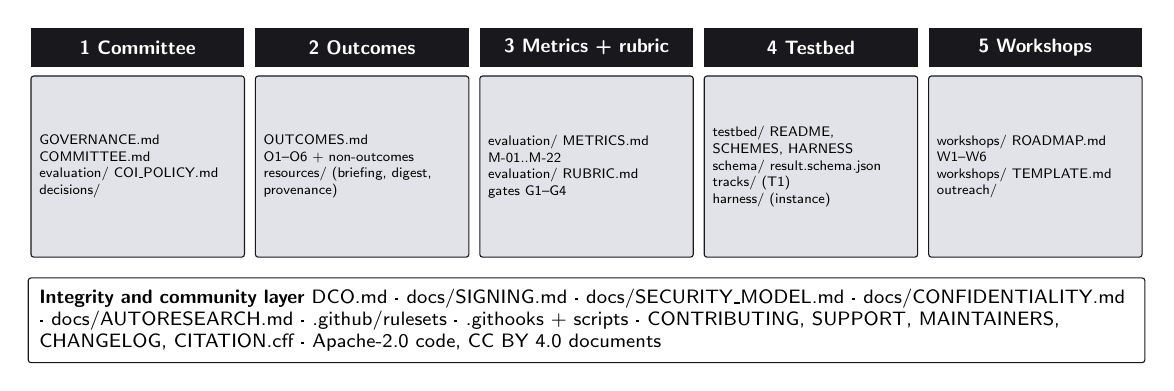
\begin{tikzpicture}[font=\scriptsize, box/.style={draw=bar,fill=lane,rounded corners=1pt,text width=2.5cm,align=left,inner sep=3pt,minimum height=2.3cm,font=\tiny}, hd/.style={fill=bar,text=white,font=\scriptsize\bfseries,text width=2.5cm,align=center,inner sep=3pt,minimum height=5mm}]
    \foreach \i/\t/\b in {
      0/1 Committee/{GOVERNANCE.md\\ COMMITTEE.md\\ evaluation/ COI\_POLICY.md\\ decisions/},
      1/2 Outcomes/{OUTCOMES.md\\ O1--O6 + non-outcomes\\ resources/ (briefing, digest, provenance)},
      2/3 Metrics + rubric/{evaluation/ METRICS.md\\ M-01..M-22\\ evaluation/ RUBRIC.md\\ gates G1--G4},
      3/4 Testbed/{testbed/ README, SCHEMES, HARNESS\\ schema/ result.schema.json\\ tracks/ (T1)\\ harness/ (instance)},
      4/5 Workshops/{workshops/ ROADMAP.md\\ W1--W6\\ workshops/ TEMPLATE.md\\ outreach/}}
      {\node[hd] (h\i) at (\i*2.85,0) {\t};
       \node[box,below=1mm of h\i] (b\i) {\b};}
    \node[draw=bar,fill=white,rounded corners=1pt,text width=13.9cm,inner sep=4pt,align=left,below=2.5mm of b2.south,anchor=north] (ev) {\textbf{Integrity and community layer} DCO.md \textperiodcentered{} docs/SIGNING.md \textperiodcentered{} docs/SECURITY\_MODEL.md \textperiodcentered{} docs/CONFIDENTIALITY.md \textperiodcentered{} docs/AUTORESEARCH.md \textperiodcentered{} .github/rulesets \textperiodcentered{} .githooks + scripts \textperiodcentered{} CONTRIBUTING, SUPPORT, MAINTAINERS, CHANGELOG, CITATION.cff \textperiodcentered{} Apache-2.0 code, CC BY 4.0 documents};
  \end{tikzpicture}
  \end{center}
  \takeaway{The README numbers the five jobs; every directory answers to one of them. Draft v0 throughout.}
\end{frame}

% ================================================================ SECTION: committee
\sectiontitle{Job 1}{Form the Evaluation Committee}{Modelled on a NIST-style process: open criteria, published rationale, reproducible results, mandatory conflict-of-interest handling.}

% ================================================================ 5 governance
\begin{frame}{Governance --- Phases and Composition}
  \begin{center}\small
  \begin{tabular}{@{}p{2.2cm}p{2.9cm}p{8.7cm}@{}}\toprule
    \textbf{Phase} & \textbf{Window} & \textbf{Output}\\ \midrule
    A --- Criteria & Sep 2026 $\rightarrow$ Jan 2027 & Outcomes ratified; metrics and rubric drafted; scheme rulings; testbed harness; COI policy; call-text inputs to the host around SSR (Dec 2026)\\
    A2 --- Pilot & Jan $\rightarrow$ Sep 2027 & Validated harness; node roster; rubric frozen before the application deadline\\
    B --- Evaluation & Nov 2027 $\rightarrow$ mid 2028 & Theoretical review track and testbed performance track; evidence set citable in standards\\
    C --- Standards & Oct 2028 $\rightarrow$ & BGIN Standard candidate $\rightarrow$ ISO/TC 307 $\rightarrow$ Japan criteria\\ \bottomrule
  \end{tabular}
  \end{center}
  {\small\textbf{Composition (proposed, 12--18 voting members):} 2 conveners \textperiodcentered{} 3--5 academia / security review \textperiodcentered{} 2--3 Bitcoin developers \textperiodcentered{} 2--3 Ethereum developers \textperiodcentered{} 2 wallet and infrastructure \textperiodcentered{} 2 measurement / testbed \textperiodcentered{} 1--2 governance / policy \textperiodcentered{} technical advisors without votes \textperiodcentered{} observers: host, NIST liaison, ISO/TC 307 liaison.}
  \takeaway{Geographic and ecosystem balance is a seating criterion. Phase A membership does not oblige Phase B.}
\end{frame}

% ================================================================ 6 decision process + COI
\begin{frame}{How Decisions Are Made --- and Kept Neutral}
  \begin{columns}[T]
    \begin{column}{0.5\textwidth}
      {\small\textbf{Decision process (GOVERNANCE \S5)}}
      \begin{enumerate}\small
        \item Discuss on Discourse --- every proposal starts as a thread
        \item Record by pull request, citing the thread and the workshop
        \item Rough consensus decides drafts; objections recorded
        \item Formal votes for: ratifying outcomes, freezing the rubric, scheme scope rulings, amending governance or COI. Simple majority, quorum of half; conveners vote only to break ties
        \item Every vote and scope ruling gets an ADR in decisions/
      \end{enumerate}
    \end{column}
    \begin{column}{0.46\textwidth}
      {\small\textbf{Neutrality (COI\_POLICY, adopt at W3)}}
      \begin{itemize}\small
        \item Mandatory COI disclosure for evaluators and node operators, published in the roster
        \item Submitters and close affiliates do not judge their round
        \item Node operators running an artifact under evaluation are recused
        \item Host funding and BGIN coordination must not compromise technical neutrality
        \item Measurement seat: node hosts are not solvers on the tracks they measure
      \end{itemize}
    \end{column}
  \end{columns}
  \takeaway{Neutrality is what makes the outputs usable as standards inputs rather than a private scorecard.}
\end{frame}

% ================================================================ SECTION: outcomes
\sectiontitle{Job 2}{Identify the Core Outcomes}{Six outcomes, each with a definition of done, the workshop that ratifies it, and an owner seat. Seeded from the METI/NEDO community briefing and the IKP-WG discussions.}

% ================================================================ 7 outcomes
\begin{frame}{Outcomes O1--O6 (draft v0, for ratification at W1)}
  \begin{center}\small
  \begin{tabular}{@{}p{0.6cm}p{4.4cm}p{6.2cm}p{2.2cm}@{}}\toprule
    & \textbf{Outcome} & \textbf{Done when} & \textbf{Ratified}\\ \midrule
    O1 & Evaluation framework in standards-ready vocabulary & METRICS and RUBRIC frozen by vote before the application deadline; every metric has a unit, method, mapping & W2; frozen A2\\
    O2 & Neutral, reproducible testbed evidence & Harness and schema adopted; $\geq$ 3 pilot nodes in 2 regions reproduce a reference run within tolerance & W3; pilot A2\\
    O3 & Crypto-agility evidence, not only readiness & Register carries switch, rollback and staged-migration metrics the testbed can execute & W2\\
    O4 & Migration-governance evidence & Governance-fit dimension with a qualitative method; open positions captured in a record & W3--W4\\
    O5 & Call-text inputs delivered to the host & Versioned package tagged; receipt acknowledged by METI/NEDO & W4\\
    O6 & Standards path & BGIN Standard outline v0; maintainer group named for Phase C & W6\\ \bottomrule
  \end{tabular}
  \end{center}
  {\scriptsize\color{soft} Non-outcomes: new primitives or parameter sets \textperiodcentered{} chain endorsement or vendor scorecards \textperiodcentered{} a Q-day date \textperiodcentered{} prize adjudication.}
\end{frame}

% ================================================================ SECTION: metrics
\sectiontitle{Job 3}{Draft the Evaluation Metrics and Rubric}{A 22-row register with units, methods and target mappings; a rubric skeleton with four gates. Written to travel: competition to BGIN Standard to ISO/TC 307 to Japan criteria.}

% ================================================================ 8 register
\begin{frame}{The Metric Register --- M-01 to M-22}
  \lead{Dual track: \textbf{(a)} theoretical security review, \textbf{(b)} implementation and performance on the testbed. Each row names the mapping it needs: BTC-tx, ETH-user, ETH-cons, L2.}
  \begin{center}\scriptsize
  \begin{tabular}{@{}p{3.1cm}p{10.7cm}@{}}\toprule
    \textbf{Group} & \textbf{Rows}\\ \midrule
    Sizes and single-op cost (b) & M-01 signature size \textperiodcentered{} M-02 public key size \textperiodcentered{} M-03 sign time \textperiodcentered{} M-04 verify time \textperiodcentered{} M-05 batch / aggregate throughput \textperiodcentered{} M-06 aggregate size\\
    Chain-level overhead (b) & M-07 per-block overhead at a reference tx mix \textperiodcentered{} M-08 mempool / gossip propagation \textperiodcentered{} M-09 block validation time \textperiodcentered{} M-10 on-chain verification gas \textperiodcentered{} M-11 state growth \textperiodcentered{} M-16 L2 / ZK verification cost \textperiodcentered{} M-17 decentralization cost\\
    Agility (a+b) & M-12 migration throughput \textperiodcentered{} M-13 rollback cost \textperiodcentered{} M-14 agility switch cost \textperiodcentered{} M-21 legacy verification continuity\\
    Review and fit (a) & M-15 wallet / UX impact \textperiodcentered{} M-19 security review score \textperiodcentered{} M-20 governance fit \textperiodcentered{} M-22 PQC-readiness claim substantiation\\
    Gate metric (b) & M-18 reproducibility --- nodes and regions reproducing the reference run within tolerance\\ \bottomrule
  \end{tabular}
  \end{center}
  \takeaway{Performance rows are scored relative to the classical baseline on the same node, never as absolute numbers. Proposed directions per row are on the register for W2.}
\end{frame}

% ================================================================ 9 rubric
\begin{frame}{The Rubric Skeleton --- Gates, Tracks, Dimensions}
  \begin{columns}[T]
    \begin{column}{0.46\textwidth}
      {\small\textbf{Gates (must pass before scoring)}}
      \begin{itemize}\small
        \item \textbf{G1 Primitive scope} --- NIST-standardized or selected, or a committee-ruled hybrid / stateful hash-based scheme
        \item \textbf{G2 Target mapping} --- evidence maps to BTC-tx, ETH-user, ETH-cons or L2
        \item \textbf{G3 Reproducibility} --- $k$ nodes, $\geq$ 2 regions, within tolerance (M-18)
        \item \textbf{G4 Disclosure} --- submitter COI disclosed; evaluators recused as required
      \end{itemize}
    \end{column}
    \begin{column}{0.5\textwidth}
      {\small\textbf{Dimensions (weights TBD at W2--W4)}}
      \begin{itemize}\small
        \item (a) assumptions, parameters, composition \textperiodcentered{} threat model \textperiodcentered{} readiness substantiation
        \item (b) verifier cost and latency \textperiodcentered{} block / mempool overhead \textperiodcentered{} on-chain and L2 cost \textperiodcentered{} decentralization cost
        \item (a+b) crypto-agility: switch, staged migration, rollback, legacy continuity
        \item (a) compatibility and wallet / UX \textperiodcentered{} governance fit
      \end{itemize}
      {\small Two evaluators per dimension; a 5-band scale with written justification; rationale published with the score.}
    \end{column}
  \end{columns}
  \takeaway{Rationale published with the score is what makes a result citable. Weights, $k$, tolerance, reference CPU class and block mix are decision records.}
\end{frame}

% ================================================================ SECTION: testbed
\sectiontitle{Job 4}{Specify the Crypto-Agility Testbed}{Servers exercising pre-existing signature schemes in Bitcoin- and Ethereum-mappable configurations. One interface, one manifest, one result schema, one reproduction protocol: that is what turns node runs into evidence.}

% ================================================================ 10 testbed concept
\begin{frame}{BSafe.network --- the Neutral Testbed}
  \begin{columns}[T]
    \begin{column}{0.5\textwidth}
      \begin{itemize}\small
        \item Geographically distributed, neutral nodes: on the order of 10--15, multi-region, multi-month runs
        \item Hosts: accredited universities, non-profits, neutral R\&D labs; contracting later under the host process
        \item Role separation: node operators are not judges
        \item Funding: initial nodes by the host; additional by contributing organizations; disclosed per node
        \item Node requirements by decision record: reference hardware class, pinned OS image and container digests, NTP and region label, operator signing key, node peering for M-08; no mainnet dependence
      \end{itemize}
    \end{column}
    \begin{column}{0.46\textwidth}
      \begin{center}\small
      \begin{tabular}{@{}p{1.3cm}p{2.2cm}p{2.6cm}@{}}\toprule
        \textbf{Phase} & \textbf{Window} & \textbf{Nodes}\\ \midrule
        T0 Spec & Sep--Nov 2026 & none; a hosted development runner for pre-flight\\
        T1 Pilot & Jan--Sep 2027 & 3--5 volunteer\\
        T2 Evaluation & Nov 2027 -- mid 2028 & 10--15 contracted\\ \bottomrule
      \end{tabular}
      \end{center}
      {\scriptsize\color{soft} Node roster: empty; offers via the \emph{Node host offer} issue template. The call opens at W3.}
    \end{column}
  \end{columns}
  \takeaway{What runs on a node: the reference harness over the scheme register, scenario runs for the chain-level metrics, and in Phase B the submitted artifacts under the same manifest.}
\end{frame}

% ================================================================ 11 schemes
\begin{frame}{The Scheme Register --- S, B and C Rows}
  \begin{center}\scriptsize
  \begin{tabular}{@{}p{1.0cm}p{4.3cm}p{3.1cm}p{5.4cm}@{}}\toprule
    \textbf{Row} & \textbf{Scheme} & \textbf{Reference} & \textbf{Status / note}\\ \midrule
    S-01 & ML-DSA (44 / 65 / 87) & FIPS 204 & candidate; the briefing's starting point\\
    S-02 & SLH-DSA (128s / 128f / 192s / 256s) & FIPS 205 & candidate; conservative, large\\
    S-03 & FN-DSA / Falcon (512 / 1024) & FIPS 206 draft & candidate; smallest lattice sigs; float risk\\
    S-04 & XMSS / XMSS\textasciicircum{}MT & SP 800-208, RFC 8391 & candidate; stateful; Poseidon2 params need a ruling\\
    S-05 & LMS / HSS & SP 800-208, RFC 8554 & candidate; stateful; state reuse = key recovery\\ \midrule
    B-01 & secp256k1 ECDSA & Bitcoin legacy / SegWit v0; ETH EOAs & baseline for BTC-tx, ETH-user\\
    B-02 & secp256k1 Schnorr & BIP-340, Taproot & baseline for BTC-tx\\
    B-03 & BLS12-381 & Ethereum consensus & baseline for ETH-cons\\ \midrule
    C-01 & Hybrid classical + PQ & IETF LAMPS direction & ruling; ``hybrid then cutover''\\
    C-02 & Quantum-resistant output type & P2QRH / BIP-360 direction & ruling; reference only, no endorsement\\
    C-03 / C-04 & Account abstraction; BLS to hash-based aggregation & Ethereum & ruling\\
    C-05 & Lattice zkVM and client-side proving & September 2026 evidence & ruling\\ \bottomrule
  \end{tabular}
  \end{center}
  \takeaway{Baselines are measured for the deltas, never as candidates. Rulings are formal votes with records.}
\end{frame}

% ================================================================ 12 harness spec
\begin{frame}{The Reference Harness --- Interface, Manifest, Reproduction}
  \pillar{0.31\textwidth}{Common interface}{Every backend exposes keygen (deterministic from seed), sign (stateful schemes expose and persist state; the leaf index is recorded), verify, sizes; batch and aggregate optional and reported as unsupported rather than absent.}\hfill
  \pillar{0.31\textwidth}{Run manifest and result}{run\_id, scheme row, parameter set, implementation (repo, commit, build flags), harness version, node (host, region, hardware fingerprint, image and container digests), fixtures, operator key --- hashed before the run; results in schema/result.schema.json.}\hfill
  \pillar{0.31\textwidth}{Reproduction protocol}{A reference run is declared; $k$ independent nodes in $\geq$ 2 regions execute the same manifest; a measurement reproduces when each node's median is within the tolerance band. The count is M-18; it feeds gate G3. Disagreements are published too.}
  \par\vspace{2mm}
  {\small\textbf{Fixtures:} 32-byte sighash-like and tx-hash-like digests plus a variable-length corpus; key sets $n \in \{1, 64, 1024, 10^5\}$; a reference block / tx mix by decision record; a legacy corpus for M-21; and (proposed) banks rather than sequences, with the instance drawn from the submission digest.}
  \takeaway{Code follows the spec, not the other way round. Implementation starts after W3 adoption.}
\end{frame}

% ================================================================ 13 open-benchmark model
\begin{frame}{Decision 0001 --- the Open-Benchmark Model for Calibration Tracks}
  \lead{Proposed for W2. The testbed is already a measuring instrument with a reproduction rule; naming a promotion rule makes it a benchmark. Calibration tracks carry no prize.}
  \begin{columns}[T]
    \begin{column}{0.5\textwidth}
      {\small\textbf{A track is one directory, one contract}}
      \begin{itemize}\small
        \item benchmark.json --- editable paths, pinned commands, score file, direction, promotion bar, runner
        \item RULES.md --- what may be edited, the score formula, the anti-overfitting rule
        \item runner.json --- the runner the score is valid on
        \item fixtures/ --- public, with provenance; promoted/ --- one directory per promotion
      \end{itemize}
    \end{column}
    \begin{column}{0.46\textwidth}
      {\small\textbf{Rules that carry}}
      \begin{itemize}\small
        \item Promotion bar = the track's reproduction tolerance; reproduced on $k$ nodes \emph{and} better than the incumbent
        \item Public note $\geq$ 5 KiB naming the exact model and harness used, or ``none''
        \item One lever per submission --- the promoted history is read by diffing
        \item Out of scope: any leaderboard of prize entries; any judgement of an applicant
      \end{itemize}
    \end{column}
  \end{columns}
  \takeaway{Whether agents are used is not the committee's to decide --- they already produce the field's numbers. Where their output is admissible, and under what attribution, is.}
\end{frame}

% ================================================================ 14 first tracks
\begin{frame}{First Tracks --- T1 Exists to Be Boring}
  \begin{center}\scriptsize
  \begin{tabular}{@{}p{2.6cm}p{5.2cm}p{5.9cm}@{}}\toprule
    \textbf{Track} & \textbf{Metric $\rightarrow$ scalar} & \textbf{Calibrates}\\ \midrule
    \textbf{T1 verify-single} (drafted) & M-04 median single verify of ML-DSA-65 over B-01, on the reference CPU class; lower is better; edit only backends/ml-dsa/; KATs pass, build pinned, no network & the reference CPU class, the tolerance band, the runner spec --- before anything harder depends on them\\
    T2 verify-batch & M-05 at $n \in \{64, 1024\}$; batch equals sequential on the same inputs & whether the register needs a batch row per scheme\\
    T3 legacy-continuity (v1) & M-21 pass / fail + cost on C-01 / C-03 paths & the ``PQC-ready chain'' continuity clause\\
    T4 agility-switch (v1) & M-14 switch cost; rollback works (M-13) & O3 evidence; whether agility is measurable at all\\ \bottomrule
  \end{tabular}
  \end{center}
  {\small\textbf{The draw as the Gap:} fixtures are banks of 65{,}536; a node times a 10{,}000-index instance drawn from the submission's own digest and a round secret it does not see. Nothing to tune to.}
  \takeaway{T1 is small, fast and fully public. Its only job is to make the reference runner real.}
\end{frame}

% ================================================================ 15 harness instance
\begin{frame}{The Calibration Harness in the Record --- harness/}
  \lead{The instrument is part of the record. harness/upstream/ vendors the agentprivacy dual-agent harness verbatim at a pinned commit (UPSTREAM.json, sha256 per file, known defects and their fixes); harness/instance/ is the pqc-calibration instance: proposer = submitter, prover = testbed node, the Gap = the fixture draw.}
  \begin{itemize}\small
    \item \textbf{Runnable as plumbing today:} the pin verifies; the vendored engine passes its own eleven gates; a stub round derives seeds and lands files; every seed and draw re-derives from the saved bytes.
    \item \textbf{Conformance fails by design} on the unmeasured baseline --- UNMEASURED until harness v0 exists; CI reports it, enforcement starts once measured.
    \item \textbf{Two defects found on the first stub round, fixed upstream the same day:} a one-byte-per-pick draw (biased for a large bank) and a one-byte seed counter; draw v2 uses 32-bit rejection-sampled picks.
    \item \textbf{What it is not:} the competition's evaluation. Prize entries are measured and attested under the host's rules and never promoted into one another.
  \end{itemize}
  \takeaway{Until real nodes are seated, every verdict is a claimed score, never a promotion. The door stays shut until the assay seat runs on a testbed node.}
\end{frame}

% ================================================================ SECTION: workshops + record
\sectiontitle{Job 5 and the record}{Run the Workshop Series; Keep the Record Honest}{Six workshops ratify jobs 1--4 before the call opens. The integrity and confidentiality layers are what let a neutral claim be checked rather than trusted.}

% ================================================================ 16 roadmap
\begin{frame}{Workshop Roadmap W1--W6, Sep 2026 $\rightarrow$ Feb 2027}
  \begin{center}\scriptsize
  \begin{tabular}{@{}p{2.4cm}p{3.6cm}p{7.7cm}@{}}\toprule
    \textbf{Workshop} & \textbf{Anchor} & \textbf{Outputs / decisions}\\ \midrule
    W1 Kickoff (late Sep) & GDC26 report; CBT session & Repository chartered; OUTCOMES ratified; governance v0; nominations open; conveners named\\
    \textbf{W2 Committee \& metrics (mid Oct)} & \textbf{Block 15}; EF Quantum Retreat; CSS / BWS & Committee seated; chairs elected; register v0 $\rightarrow$ v1; scheme scope rulings; open questions 1--5 assigned; ruling on decision 0001\\
    W3 Testbed (Nov) & CSS / BWS drafting & Harness interface and schema adopted; reference CPU class and block mix; COI policy adopted; node-host call; T1 opened if 0001 passed; 0002 = $k$ + tolerance\\
    W4 Rubric \& call text (Dec) & SSR PQC workshop, 13 Dec, Baltimore & Rubric v1; ``PQC-ready chain'' v1; call-text package tagged and delivered (O5)\\
    W5 Pilot (Jan) & Applications open (planned) & 3--5 pilot nodes; tolerance calibrated; rubric v1.1\\
    W6 Retrospective (Feb) & CoDecFin 2027 at FC'27 & Phase A retrospective; A2 / B confirmed; BGIN Standard outline v0 (O6); maintainers named\\ \bottomrule
  \end{tabular}
  \end{center}
  \takeaway{Each session rides an existing calendar anchor. Conveners publish a status on Discourse after each workshop, linking the record.}
\end{frame}

% ================================================================ 17 integrity
\begin{frame}{Integrity --- Why Every Action Carries a Signature}
  \begin{columns}[T]
    \begin{column}{0.5\textwidth}
      {\small\textbf{Baseline controls}}
      \begin{itemize}\small
        \item DCO sign-off on every commit: web setting, client hook, CI job matching sign-off to author
        \item Cryptographic signatures required on every branch and tag, no bypass; .allowed\_signers for offline verification
        \item main: PR-only, three required checks, linear history, no force-push, no deletion, no admin bypass
        \item Merged by fast-forward push of the signed head --- never the squash or rebase buttons
        \item Actions SHA-pinned, read-only; Dependabot weekly; OpenSSF Scorecard
      \end{itemize}
    \end{column}
    \begin{column}{0.46\textwidth}
      {\small\textbf{What the controls caught}}
      \begin{itemize}\small
        \item The first four merges used GitHub's squash button: GitHub-signed commits, three without sign-off --- rejected by the history check
        \item main rebuilt the same hour from the PRs' signed heads: identical tree, verify-history clean
        \item Approvals 1 $\rightarrow$ 0 while one convener is seated; restored with the second
      \end{itemize}
      {\small Every commit and tag on main is signed and signed-off by a named contributor; the whole history verifies offline.}
    \end{column}
  \end{columns}
  \takeaway{A neutral record is worth citing only if anyone can verify who wrote it.}
\end{frame}

% ================================================================ 18 confidentiality
\begin{frame}{What Is Held Back, and Why --- the Public Rule}
  \lead{The default is publication. Material is held only if at least one of four tests is true; the rule is public even when the material is not. Held material lives in a separate access-controlled repository readable by the conveners and the seated committee.}
  \begin{center}\small
  \begin{tabular}{@{}p{3.6cm}p{5.6cm}p{4.4cm}@{}}\toprule
    \textbf{Test} & \textbf{Meaning} & \textbf{What is published instead}\\ \midrule
    Not ours to publish & Circulated without clearance; Chatham House; third-party rights & The fact and the provenance row\\
    Names a person deliberatively & A nomination, a COI disclosure, a score before announcement & The seated roster row; the fact of a recusal\\
    Would pre-empt an announcement & Draft call text before the host publishes it & The tagged package once acknowledged\\
    Arrived under terms & Applicant material; results tied to a named operator & What the host allows\\ \bottomrule
  \end{tabular}
  \end{center}
  \takeaway{Unfinished is not confidential. Awkward is not confidential. Disagreement about a metric, a scheme, a date or a ruling is public work.}
\end{frame}

% ================================================================ 19 outreach + resources
\begin{frame}{Outreach and Sources --- What Was Said, and Where It Came From}
  \begin{columns}[T]
    \begin{column}{0.5\textwidth}
      {\small\textbf{Public channel (since 11 Sep 2026)}}
      \begin{itemize}\small
        \item The \emph{Post-Quantum Crypto Agility Competition} category on the BGIN Discourse: launch, workshop series, committee nominations; replies on the IKP PQC and GDC26 threads
        \item Held for the committee's week: the metric and scheme call for comment; the node-host call
        \item bgin-global.org/projects/pqc-migration carries the competition: repository, the category, the GDC26 scene-setting deck and the PRX Quantum paper
        \item House style: no salutation; the post carries the ask and the link, the repository the detail; nothing announced as settled before ratification
      \end{itemize}
    \end{column}
    \begin{column}{0.46\textwidth}
      {\small\textbf{Resources with provenance}}
      \begin{itemize}\small
        \item METI/NEDO community briefing (July 2026) and its digest
        \item Google Quantum AI et al., PRX Quantum 7, 031001 --- DOI, arXiv, ePrint
        \item GDC26 meeting report and scene-setting deck (hosted on the BGIN site)
        \item Project Eleven, state-reuse key recovery (Sep 2026)
        \item PQC Audit Index: FIPS 206 status, LMS sizes, M-19 checklist seeds, migration timelines
        \item BIP-340; BIP-360 direction --- reference only
      \end{itemize}
    \end{column}
  \end{columns}
  \takeaway{Every claim that has a source names it; where sources disagree, both are carried and attributed.}
\end{frame}

% ================================================================ 20 status + open doors
\begin{frame}{Status at Block 15 --- and What Is Open}
  \begin{columns}[T]
    \begin{column}{0.48\textwidth}
      {\small\textbf{In the record (main, signed, CI green)}}
      \begin{itemize}\small
        \item Charter: README, governance, roster, outcomes, contributing
        \item Evaluation: register M-01..M-22 with proposed directions, rubric skeleton, COI policy
        \item Testbed: node model, scheme register, harness spec, result schema, T1 track contract, calibration harness instance
        \item Roadmap W1--W6; decision 0001 proposed; confidentiality rule; outreach record; resources
      \end{itemize}
    \end{column}
    \begin{column}{0.48\textwidth}
      {\small\textbf{Open doors}}
      \begin{itemize}\small
        \item \textbf{Second convener} --- the reason approvals sit at 0; onboarding is docs/SIGNING.md
        \item \textbf{Nominations} --- open; seats across academia, Bitcoin, Ethereum, wallets, measurement, governance
        \item \textbf{Node hosts} --- the call opens at W3; the roster is empty
        \item \textbf{SSR paper} --- 12 Oct deadline; the repository holds a competition-design contribution
        \item \textbf{Decision records} --- 0001 at W2; 0002 ($k$, tolerance, reference class) at W3
      \end{itemize}
    \end{column}
  \end{columns}
  \takeaway{Twenty-two signed commits, one convener, zero nominations confirmed. The record is ahead of the committee --- Block 15 is where that inverts.}
\end{frame}

% ================================================================ 21 contribute
\begin{frame}{How to Contribute --- Thread, Issue, Pull Request}
  \begin{columns}[T]
    \begin{column}{0.55\textwidth}
      \begin{enumerate}\small
        \item \textbf{Discuss} on the Discourse category; every proposal starts as a thread
        \item \textbf{Open an issue} from a template: source, metric, scheme, node-host offer, committee nomination
        \item \textbf{Pull request}, signed and signed-off --- one-time setup with scripts/setup-signing.sh; docs/SIGNING.md walks it
        \item \textbf{Land it} by fast-forward push of the signed head after review; the CHANGELOG records it per signed tag
      \end{enumerate}
      {\small Documents CC BY 4.0; code Apache-2.0; Contributor Covenant 2.1. Cite a tagged version via CITATION.cff.}
    \end{column}
    \begin{column}{0.42\textwidth}
      \begin{center}\tiny
        \begin{tabular}{@{}>{\centering\arraybackslash}p{2.6cm}@{\hspace{3mm}}>{\centering\arraybackslash}p{2.6cm}@{}}
          \qrcode[height=1.6cm]{https://github.com/bgin-global/pqc-agility-competition} & \qrcode[height=1.6cm]{https://bgin.discourse.group/c/post-quantum-crypto-agility-competition/44} \\[0.5mm]
          \textbf{Repository} & \textbf{Discourse category} \\
          github.com/bgin-global/ pqc-agility-competition & bgin.discourse.group/c/ post-quantum-crypto-agility-competition/44
        \end{tabular}
      \end{center}
    \end{column}
  \end{columns}
  \takeaway{Nothing here is final until the evaluation committee ratifies it and the host publishes the official call.}
\end{frame}

% ================================================================ CLOSE
{\setbeamertemplate{footline}{}
\begin{frame}[plain]
  \begin{tikzpicture}[remember picture,overlay]
    \fill[bar] (current page.north west) rectangle (current page.south east);
    \node[anchor=south,text=white,font=\Large\bfseries,text width=13.5cm,align=center,execute at begin node=\nohyph] at ([yshift=6mm]current page.center){The repository is the record.};
    \node[anchor=north,text=white,font=\small,text width=13.5cm,align=center,execute at begin node=\nohyph] at ([yshift=3mm]current page.center){Decisions, drafts, sources, and testbed specifications --- signed, public, and draft v0 until ratified.};
    \node[anchor=north,text=soft,font=\small,text width=13.5cm,align=center,execute at begin node=\nohyph] at ([yshift=-9mm]current page.center){github.com/bgin-global/pqc-agility-competition \textperiodcentered{} Post-Quantum Crypto Agility Competition category on the BGIN Discourse};
    \node[anchor=south east,inner sep=0] at ([xshift=-7mm,yshift=5mm]current page.south east){
\includegraphics[height=1.4cm]{bgin_logo.png}};
  \end{tikzpicture}
\end{frame}}

\end{document}
